\documentclass[12pt, letterpaper]{article}
\usepackage[utf8]{inputenc}
\usepackage[spanish]{babel}
\usepackage{graphicx, fancyhdr}
\usepackage[colorlinks, linkcolor = teal]{hyperref}
\usepackage[top = 2cm, bottom = 6cm, textwidth = 13cm]{geometry}
\usepackage[all]{background}
\usepackage{float}
%\usepackage{subfiles}
%\usepackage{booktabs}
%\usepackage{pgfplots}
%\usepackage{siunitx}
%\usepackage[hyphens]{url}

\SetBgContents{\underline{\makebox[0.5cm][1]{}Reporte de Práctica, Formación Dual, Continental-UAQ.\makebox[7.3cm][1]{}}}    % Set contents
\SetBgPosition{13cm, -8.3cm}        % Select location
\SetBgOpacity{1}                    % Select opacity
\SetBgAngle{90}                     % Select rotation of logo
\SetBgScale{1.3}                    % Select scale factor of logo

\fancypagestyle{plain}{
    \fancyhf{}        % Clear header/footer
    \fancyhead[L]{
\includegraphics[height = 60pt, keepaspectratio = true]{img/header/Escudo-UAQ.png}}
    \fancyhead[C]{
\includegraphics[height = 50pt, keepaspectratio = true]{img/header/FI-btm-pd.png}}
    \fancyhead[R]{
\includegraphics[height = 60pt, keepaspectratio = true]{img/header/Escudo-FI.png}}
    \fancyfoot[R]{\thepage}
    \fancyfoot[L]{Reporte de Práctica}
    \renewcommand{\headrulewidth}{0pt}
    \setlength{\headheight}{65pt}
}
\pagestyle{plain}   % Set page style to plain.


\title{\bf UNIVERSIDAD AUTÓNOMA DE QUERÉTARO \& CONTINENTAL Co.\\
\hfill \\
\large COMUNICACIÓN SCI ENTRE DOS TARJETAS DELFINO UTILIZANDO 
CONTROL DE VERSIONES \\ \rule[2mm]{130mm}{0.5mm}\\
\begin{flushleft}
    \hfill \\
    Programa de educación DUAL Continental-UAQ\\
    Semestre: 2020B\\
    \hfill \\
    \large{TUTORES: \\} 
\end{flushleft}
\hfill \\ \hfill \\
M. Alejandro Rivera Garay\\Dr. Mariano Garduño Aparicio\\
\begin{flushleft}
    \hfill \\
    \large{ALUMNOS: \\}
\end{flushleft}
}
         
\author{\small Iván Eduardo Andrade Jains
\and 
\small Andrea Abigail Anievas Guerrero
\and 
\small Farid Iván Arriaga Tejeda
\and 
\small Luis Ángel Chávez Espínola
\and 
\small Rubén Alejandro García Sánchez
\and 
\small Jesús Alberto Herrera Curiel
\and
\small Claudia Beatriz Reséndiz Jurado
\and 
\small Gabriela Suárez Páez
\and 
\small Mayra Denisse Uribe Escobar}                        
\date{\today}                          
\begin{document}
\maketitle
%\tableofcontents

\pagebreak

\section{INTRODUCCIÓN}

\subsection{Comunicación serial}
La comunicación serie o comunicación secuencial, es el proceso de envío de datos de un bit a la vez, de forma secuencial, sobre un canal de comunicación o un bus.\\
Las características más importantes de la comunicación son:

\begin{itemize}
    \item Velocidad de transmisión
    \item Bits de datos
    \item Bits de parada
    \item Bit de paridad
\end{itemize}

Para que dos puertos puedan comunicar es necesario que las características sean iguales. La velocidad de transmisión indica el número de bytes por segundo que se transfieren y se miden en baudios(bauds) \cite{DATA}.\\
Ancii es una herramienta para comunicarse por medio de comunicación serial, existe ancii estándar(0 a 127) es decir utiliza 7 bits y ancii extendido(0 a 255) por lo que utiliza 8 bits, un paquete se refiere a una transferencia de base Incluyendo los bits de inicio y parada así como los datos bit de datos debido a que el número actual de bits depende en el protocolo que se selecciona el término paquete se usa para referirse a todos estos casos \cite{ASCII}.\\
Además, me comunicación serial puede ser utilizada para adquisición de datos si se usa un conjunto con un dispositivo remoto de muestreo el puerto serial recibe y envía datos envía bit de información un bit a la vez aún y cuando esto es más lento Que la comunicación en paralelo que permiten la transmisión de un by completo por este método de comunicación es más sencillo y puede alcanzar mayores distancias.

\subsection{GIT}
Git es un software de control de cambios en diferentes versiones de un código. Git permite realizar un seguimiento de los cambios en archivos y, si es necesario, restaurar las versiones anteriores. El uso de Git permite a varias personas trabajar simultáneamente en el mismo código sin tener que sobrescribir los cambios del otro.\\
Además, Git permite la creación de múltiples alternativas. Estas versiones se pueden utilizar para probar nuevos plugins y estructuras de sitios web o para el desarrollo independiente de varios scripts PHP.

\subsection{Interfaz de Comunicación Serial de la tarjeta F28377S}
El módulo de la Interfaz de Comunicación Serial, o por sus siglas en ingles SCI (Serial Communication Interface), es un puerto de Entradas y Salidas en serie que hace posible la comunicación asincrónica entre la tarjeta F28377S y otros dispositivos periféricos. Usualmente se le conoce por sus siglas en inglés como UART (Universal Asynchronous Receiver Transmitter) y es utilizado comúnmente de acuerdo al estándar de comunicación RS232.\\
El transmisor y receptor del SCI cuentan con un FIFO de 16 palabras, cada uno con sus propios bits de habilitación e interrupción. Ambos pueden ser operados de forma independiente para comunicaciones Half-Duplex, o de forma simultánea para comunicaciones Full-Duplex. La tasa de bits es programable para diferentes velocidades de comunicación a través de un registro de 16 bits.

\begin{figure}[H]
    \centering
    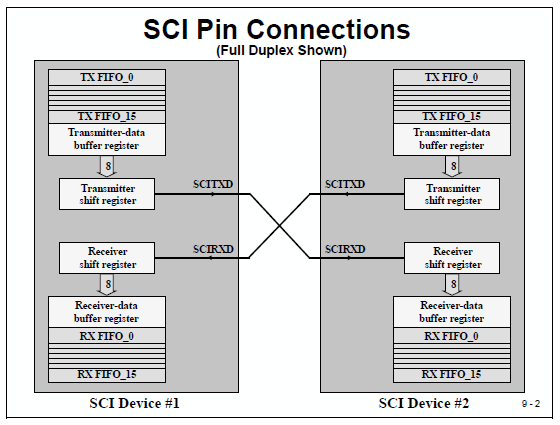
\includegraphics[width=0.75\textwidth]{img/intro/SCI_PIN.png}
    \caption{Diagrama de composición del SCI para una comunicación Full Duplex}
\end{figure}
\pagebreak

\section{OBJETIVO}

Con el entendimiento del funcionamiento del código para comunicación SCI, realizar la conexión y la comunicación entre dos tarjetas Delfino tomando en consideración los requisitos expuestos por el profesor utilizando Git como principal herramienta para control de versiones.

\section{MATERIAL}

A continuación, se enlista el material utilizado para la realización de la práctica:
\begin{itemize}
    \item 2 tarjetas Delfino LaunchPad – LaunchXL-F28377S
    \item 3 cables DuPont Hembra Hembra
\end{itemize}

\section{DESARROLLO}

\subsection{Descripción del código}
Para el desarrollo de esta práctica se empleó parte del código que hicimos anteriormente para que entre dos tarjetas se comunicaran y formaran la palabra “Hola”. Como en esta ocasión no se requería únicamente de caracteres, se optó por utilizar un número concreto de strings en el vector msg, en cuánto a las funciones se emplearon las mismas con las que ya habíamos venido trabajando, sin embargo, se sumó una llamada “scic\_rcv\_msg”, tal y como se puede observar en la siguiente imagen.

\begin{figure}[H]
    \centering
    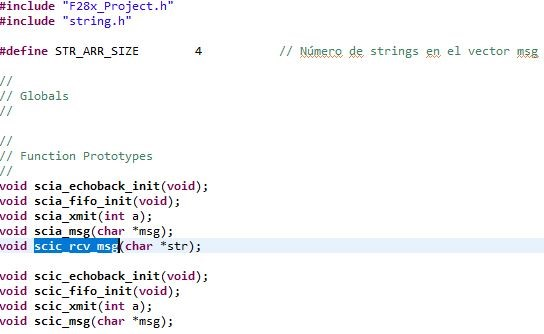
\includegraphics[width=0.75\textwidth]{img/desarrollo/DES_1.jpg}
    \caption{Declaración de funciones.}
\end{figure}

Posteriormente llegamos al main del programa, en esta parte declaramos dos contadores, uno llamado i que es empleado para avanzar en el array msg y con el contador it que es el encargado de que el programa se ejecute únicamente 10 ocasiones, también se declara el string que será usado para almacenar lo que se recibe a través del puerto SCIC y está el vector que contiene las palabras con las que se compararán los mensajes recibidos y los mensajes que deben enviarse, adicionalmente se inicializan los puertos de comunicación SCIA y SCIC, sin embargo no se dará una explicación a profundidad de dichas cuestiones puesto que en el código anterior fueron utilizadas de igual forma.

\begin{figure}[H]
    \centering
    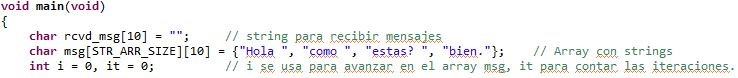
\includegraphics[width=0.75\textwidth]{img/desarrollo/DES_2.jpg}
    \caption{Declaración de contadores y variables tipo char.}
\end{figure}

Dentro del main también se encuentra la lógica principal del programa, donde únicamente se ejecuta 10 veces y al término de estas 10 veces se envía el mensaje “Fin”, dentro del main se hace llamar a la función scic\_rcv\_msg y a su vez obtener el valor que contendrá la variable rcvd\_msg. Posteriormente se hará una explicación detallada de dicha función. Tras haber obtenido el valor de la variable rcvd\_msg se realiza una comparación con la variable msg que contiene las palabras con las que se va a formar la oración y se selecciona la posición del vector mediante el contador i que dependiendo de la iteración en la que nos encontremos irá cambiando y esperará la palabra correspondiente a la iteración en la que se encuentra. Si la palabra que se recibe es igual a la palabra en el vector el comando strcmp arroja un cero, en caso de que sean iguales se procede a imprimir por el SCIA en la consola del CCS la palabra recibida, se da un delay de 2 segundos según lo establecido por el Dr. Mariano y se procede a enviar la palabra del vector en la posición correspondiente, en el momento en que el contador i supera el valor de la cantidad de palabras almacenadas en el vector, se reinicia a 0 y a su vez se aumenta en uno el contador it. Una vez finiquitadas las 10 iteaciones, se sale del ciclo while y se envía por el puerto SCIA la palabra Fin.

\begin{figure}[H]
    \centering
    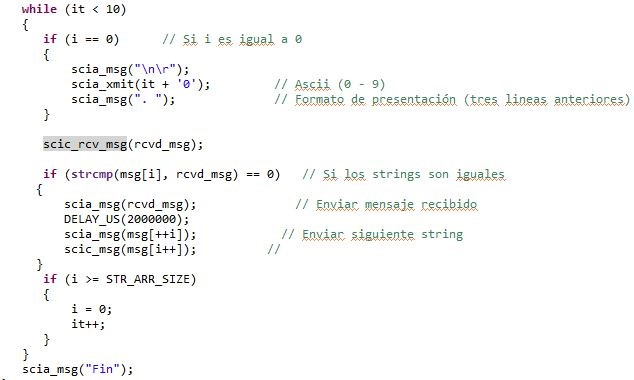
\includegraphics[width=0.75\textwidth]{img/desarrollo/DES_3.jpg}
    \caption{Estructura lógica principal del programa.}
\end{figure}

Por último, tenemos la función scic\_rcv\_msg, la cual se encarga de recibir la trama de datos que forma la palabra que se ha enviado a través de la otra tarjeta. Su funcionamiento se explica en la siguiente figura.

\begin{figure}[H]
    \centering
    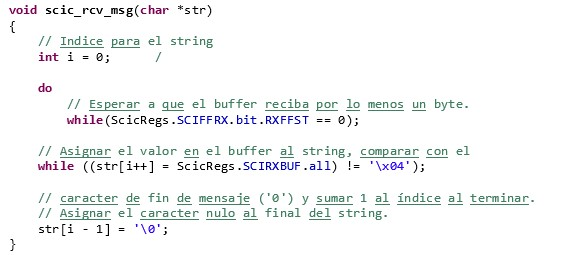
\includegraphics[width=0.75\textwidth]{img/desarrollo/DES_4.jpg}
    \caption{Código de la función para recibir strings.}
\end{figure}

El resto del código está constituido por las funciones previamente empleadas y estudiadas, como lo son las funciones para configurar la velocidad de comunicación y la forma en la que va a estar constituida la trama de datos. Solo queda agregar que se hizo una pequeña modificación a la función scic\_msg la cual es la encargada de transmitir la trama de datos a través del puerto SCIC, se hizo que tras enviar el mensaje enviara también el valor hexadecimal 04, que equivale a un 4 en decimal y si se observa la tabla ASCII se podrá constatar que es el carácter que indica el fin de la transmisión, carácter que es empleado en la función scic\_rcv\_msg para encontrar el final de la trama de datos.\\
En caso de requerir mas detalle sobre los códigos favor de consultar los archivos anexos correspondientes a los códigos.

\subsection{Conexiones realizadas}
Utilizando la documentación de la tarjeta se determinó la posición de los pines correspondientes al módulo SCIC para realizar la interconexión de las tarjetas.

\begin{figure}[H]
    \centering
    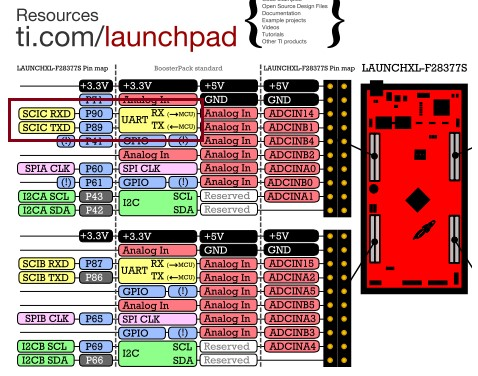
\includegraphics[width=0.75\textwidth]{img/desarrollo/PIN_MAP.jpg}
    \caption{Los pines 3 y 4 de J1 de la tarjeta son los correspondientes al módulo SCIC.}
\end{figure}

\subsection{Resultados}
Una vez que se realizó la conexión física, se procedió a cargar los códigos correspondientes a cada tarjeta. Ya con el código cargado en cada tarjeta, se utilizó la terminal de Code Composer para observar los resultados obtenidos y así visualizar la información que estaba transmitiéndose y recibiéndose en cada una de las tarjetas.

\begin{figure}[H]
    \centering
    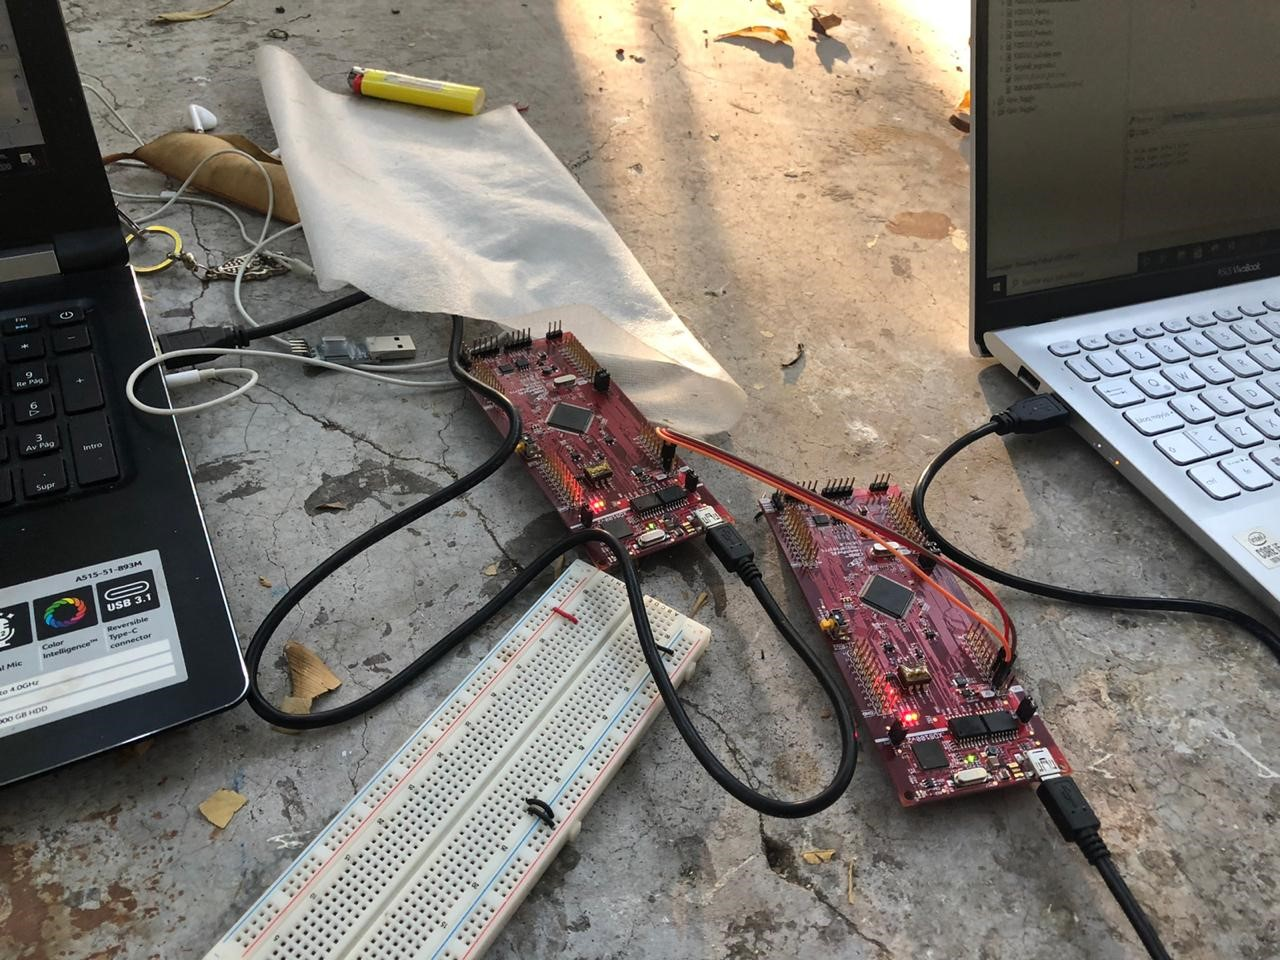
\includegraphics[width=0.75\textwidth]{img/desarrollo/RES_1.jpg}
    \caption{Conexión del puerto SCIC en ambas tarjetas.}
\end{figure}

Como se observa en las figuras siguientes, los resultados fueron los esperados y la comunicación entre las tarjetas fue exitosa.

\begin{figure}[H]
    \centering
    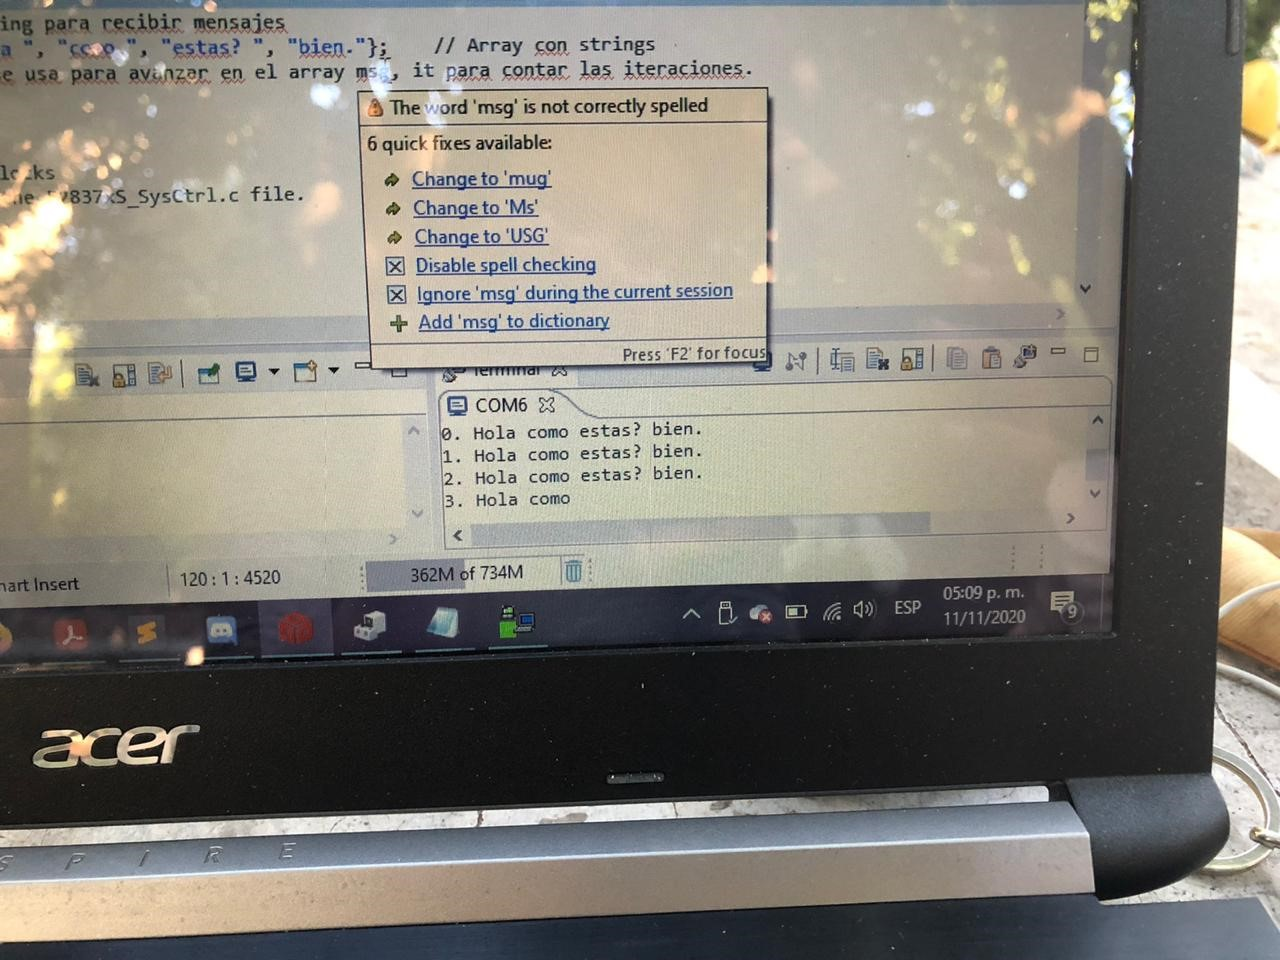
\includegraphics[width=0.75\textwidth]{img/desarrollo/RES_2.jpg}
    \caption{Terminal serial de Code Composer, desplegando la información enviada y recibida en la Tarjeta A.}
\end{figure}

\begin{figure}[H]
    \centering
    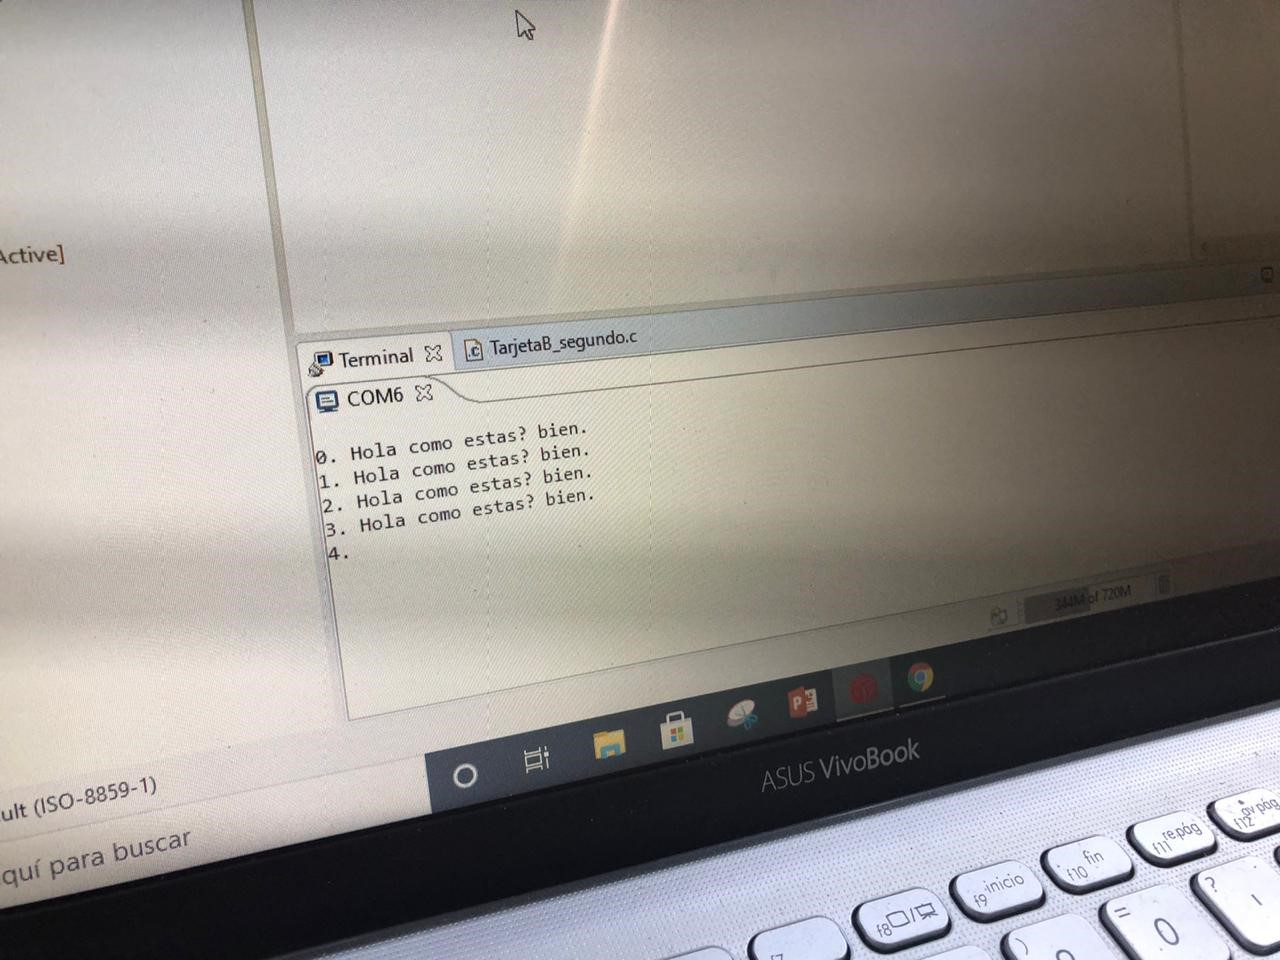
\includegraphics[width=0.75\textwidth]{img/desarrollo/RES_3.jpg}
    \caption{Terminal serial de Code Composer, desplegando la información enviada y recibida en la Tarjeta B.}
\end{figure}

A continuación, se muestran los network graph de GitHub correspondientes al repositorio del código y al repositorio de la práctica.

\begin{figure}[H]
    \centering
    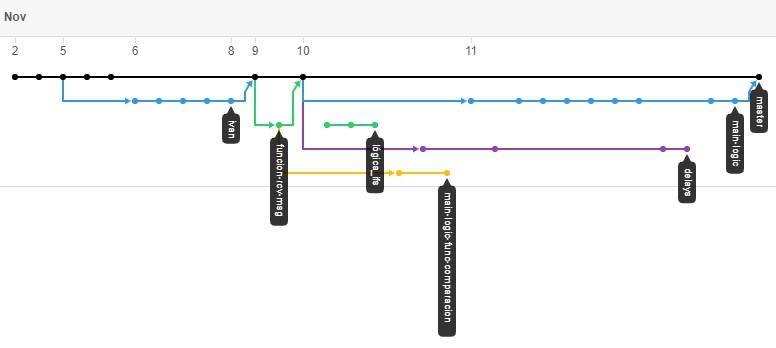
\includegraphics[width=0.75\textwidth]{img/desarrollo/CODE_NETWORK.jpg}
    \caption{Network Graph correspondiente al repositorio del código.}
\end{figure}

\begin{figure}[H]
    \centering
    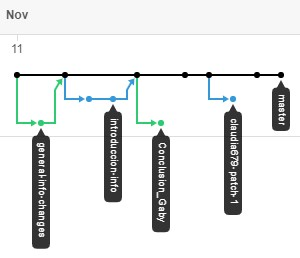
\includegraphics[width=0.75\textwidth]{img/desarrollo/DOC_NETWORK.jpg}
    \caption{Network Graph correspondiente al repositorio del reporte.}
\end{figure}

El video de los resultados se encuentra en los anexos a este reporte.
\pagebreak

\section{CONCLUSIONES}
Iván: Iván Eduardo Andrade Jains \\
Andrea: \\
Farid: \\
Luis: \\
Rubén: \\
Jesús: \\
Claudia: \\
Gabriela: \\
Mayra: \\
\pagebreak

\begin{thebibliography}{2}
    \bibitem{DATA}
    Catthoor, F., Danckart, K., Kulkarni, C.
    (2002). 
    \textit{Data access and storage management for embedded programmable processors.} 
    Boston: Kluwer Academic.

    \bibitem{ASCII}
    Heslop K., Karst J., Prensky S., Schmitt D.
    (2000).
    \textit{LAS 3.0. Log ASCII Standard.}
    Calgary, Alberta.
\end{thebibliography}

\end{document}